\documentclass[]{article}
\usepackage{amsmath}
\usepackage{graphicx}
%\usepackage{xcolor}
\usepackage{hyperref}
\usepackage[dvipsnames]{xcolor}
\usepackage{matlab-prettifier}
\usepackage{fullpage}

\graphicspath{ {images/} }

% Title Page
\title{Laboratory 4: Face Detection by the Viola-Jones' algorithm and deep-learning}
\author{Jesus Miguel Adrian Matos}
\date{\today}


\begin{document}
	\maketitle
	
	\begin{abstract}
		\noindent This laboratory deals with face detection algorithms. 		
\noindent The work is organised as follows:
\begin{itemize}
\item Section 1: we explain the inputs.
\item Section 2: we explain the outputs and its structure of the results, and the shape of the resulting matrix
\item Section 3: we explain the code for ViolaJones.
%\item Section 4: we report the listing of the codes 
%\item Section 4: we explain .
\end{itemize}
		
		%con los conocimientos de clase
		%En la parte 1 explicamos las entradas para poder conseguir la estructura de movimiento. 
		%En la parte 2 calculamos la estructura del resultado, que es la forma de la matriz. 
		%
		%using Matlab software y los conocimientos de clase
		%En la parte 3 explicamos el codigo para calcular la estructura para un cuerpo Rigid structure from motion by factorization.
		%En la parte 4 explicamos el codigo para calcular la estructura para un cuerpo Non-Rigid structure from motion by non-linear optimization and assuming a low- rank shape model.
		%En la parte 5 explicamos el codigo para calcular la estructura para un cuerpo Non-Rigid structure from motion by factorization and assuming a low-rank trajectory model.
		
		
	\end{abstract}
	
	%\newpage 
	
	\input{inputs}
	\section{Outputs:}
The code returns us a matrix $[x\, y\, width\, height]$ with a dimension of $n\times 4$ of the detected objects such that:
\begin{itemize}
	\item $n$: Number of objects detected.
	\item $x$: Coordinate of the row, where the object in the image begins.
	\item $y$: Coordinate of the column, where the object in the image begins. %
	\item $width$: Width of the detected object.
	\item $height$: Height of the detected object.
\end{itemize}
We will call each row of this matrix \textbf{Rectangle} $Rectangle^{i}$. In figure \ref{fig:rect} we can see the example of a $Rectangle^{i}$ matrix within an image.
\begin{figure}[h!]
	\centering
	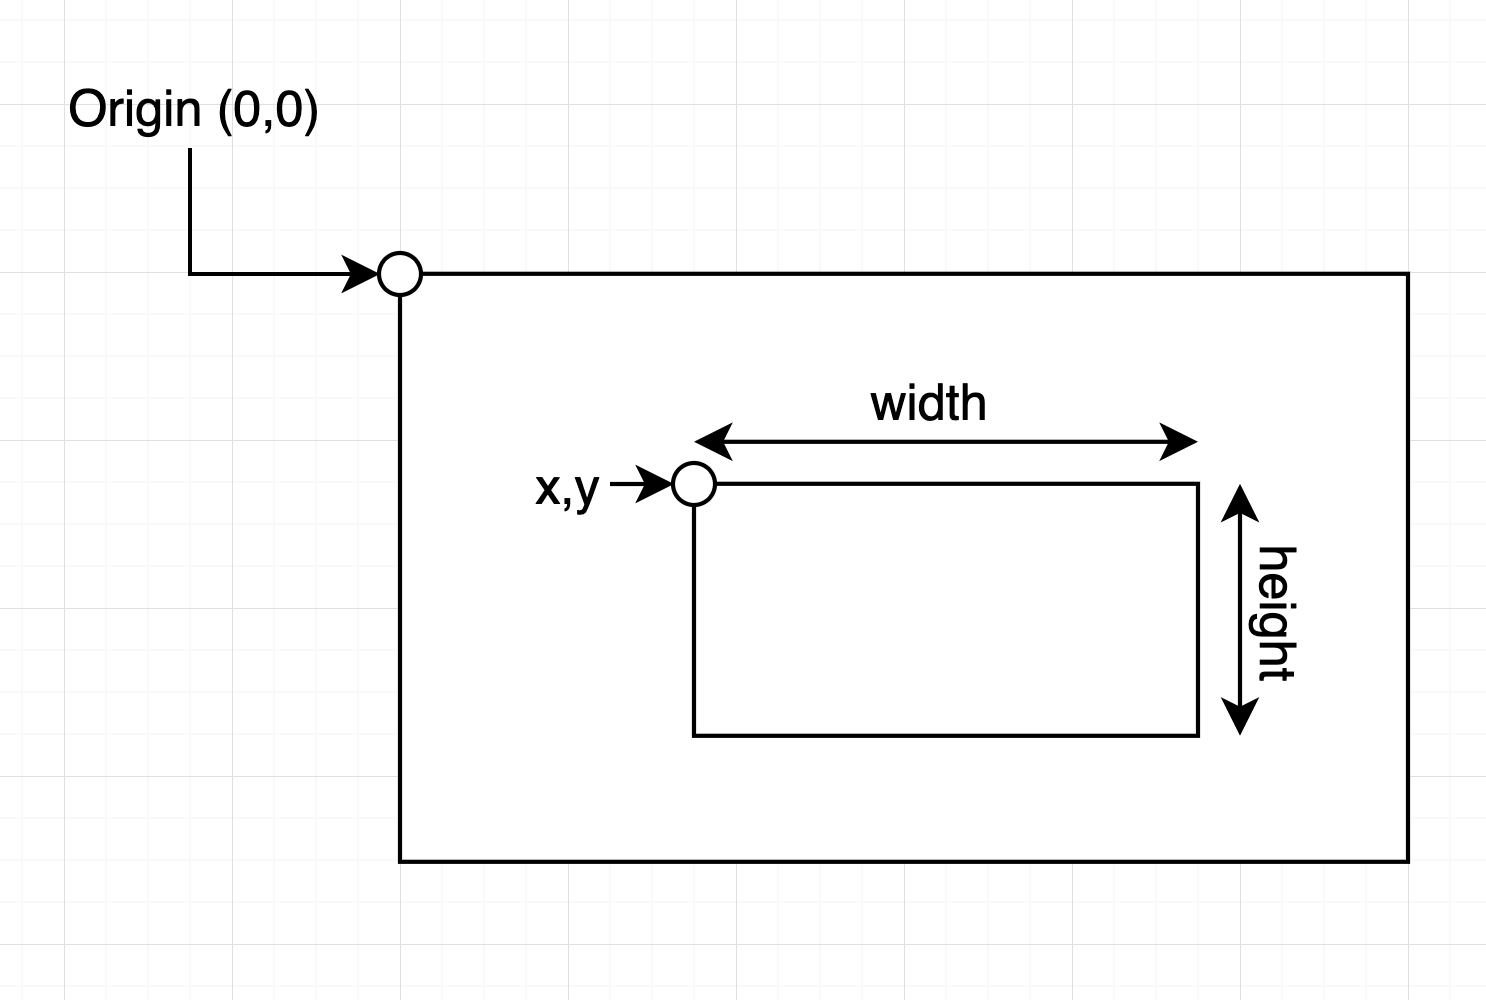
\includegraphics[scale=0.3]{T1/rectangle}
	\caption{$Rectangle^{i}$ matrix.}
	\label{fig:rect}
\end{figure}
	\section{First Part (ViolaJones):}
The code for Viola Jones is composed by the following files
\begin{itemize}
	\item \textbf{ConvertHaarcasadeXMLOpenCV.m}: This function is required to translate OpenCV feature functions from XML to syntax Matlab in order to be compiled.
	\item \textbf{ObjectDetection.m}: This is the beginning of the detection, where the input parameters are received and invokes the functions \textbf{GetIntergralImages.m} and  \textbf{HaarCasadeObjectDetection.m}.
\item \textbf{GetIntergralImages.m}: This function computes the \textbf{integral matrix} for the image.
\item \textbf{HaarCasadeObjectDetection.m}: This function uses the Cascade Classifier to calculate the \textbf{Rectangle} matrices. 
\end{itemize}

\subsection{Code:}
\noindent Let start by describing what is important about the codes.\\
\noindent The first code called is \textbf{ObjectDetection.m} Listing \ref{lst:ObjectDetection}.\\%xq primero listing2? 
\noindent On line 3 of the Listing \ref{lst:ObjectDetection}, we have the default options:
\begin{itemize}
	\item \textbf{ScaleUpdate}: This tells us that the scale of the current \textbf{window} will increase from 1 to 1.2 in each iteration. Thus, if the current scale is $X$, the next scale will be $1.2X$. 
	\item \textbf{Resize}: Resizes the image so that the longest side (width or height) is equal to 384.
	\item \textbf{Verbose}: To show the calculations of the iterations.
\end{itemize}

\noindent On line 31 of the Listing \ref{lst:ObjectDetection}, we load the image and convert it into an array, but if the image is coloured then the pixels of the array has 3 values in each pixel $(r,g,v)$.\\

\noindent On line 35 of the Listing \ref{lst:ObjectDetection}, this function extracts the feature functions already trained by \textbf{OpenCV}, which are our \textbf{Strong Classifiers} when examining each \textbf{window}, as shown in lecture slide in Figure \ref{fig:slideT1}.\\

\noindent On line 37 of the Listing \ref{lst:ObjectDetection},we compute the \textbf{integral matrix} using the function \textbf{GetIntergralImages.m} (see Listing \ref{lst:GetIntergralImages}).\\ 

\noindent On line 1 of the Listing \ref{lst:GetIntergralImages}, we convert the image array to a double-type.\\

\noindent On lines from 2 to 12 of the Listing \ref{lst:GetIntergralImages}, the image resize mentioned is performed (option resize). The reason for the ratio between the real size of the image and its current size is saved $Ratio=size(Picture,2)/384$.\\


\noindent On lines from 14 to 16 of the Listing \ref{lst:GetIntergralImages}, here we convert the image to garyscale, which means, that our pixels no longer have 3 values (r,g,b) buy have a single value.\\

\noindent On lines from 18 to 39 of the Listing \ref{lst:GetIntergralImages}, here we compute the \textbf{integral matrix} for the image, in the Figure \ref{fig:integral} you can see how compute the  \textbf{integral matrix}.

\noindent On lines from 41 to 62 of the Listing \ref{lst:GetIntergralImages}, here we compute the \textbf{integral matrix} for $I2$, where $I2$ is
\begin{equation}
	\text{let }	I=
	\begin{pmatrix}
		i_{11} & i_{12} & \cdots & i_{1n}\\
		i_{21} & i_{22} & \cdots & i_{2n}\\
		\vdots & \vdots & \ddots & \vdots\\
		i_{m1} & i_{m2} & \cdots & i_{mn}\\
	\end{pmatrix}
	\Rightarrow I2=
	\begin{pmatrix}
		(i_{11})^2 & (i_{12})^2 & \cdots & (i_{1n})^2\\
		(i_{21})^2 & (i_{22})^2 & \cdots & (i_{2n})^2\\
		\vdots & \vdots & \ddots & \vdots\\
		(i_{m1})^2 & (i_{m2})^2 & \cdots & (i_{mn})^{2}\\
	\end{pmatrix}
\end{equation}

\noindent On lines from 64 to 66 of the Listing \ref{lst:GetIntergralImages}, here we only add the \textbf{height} and \textbf{width} of the current image (with a maximum side like 384), and the \textbf{ratio} of change of the image resize to structure $IntegralImages$.





\noindent On line 39 of the Listing \ref{lst:ObjectDetection}, we call the function $HaarCasadeObjectDetection$, which applies cascade classification to find the \textbf{Rectangle} matrices that contain the faces that appear in the image.

\begin{figure}[h]
	\centering
	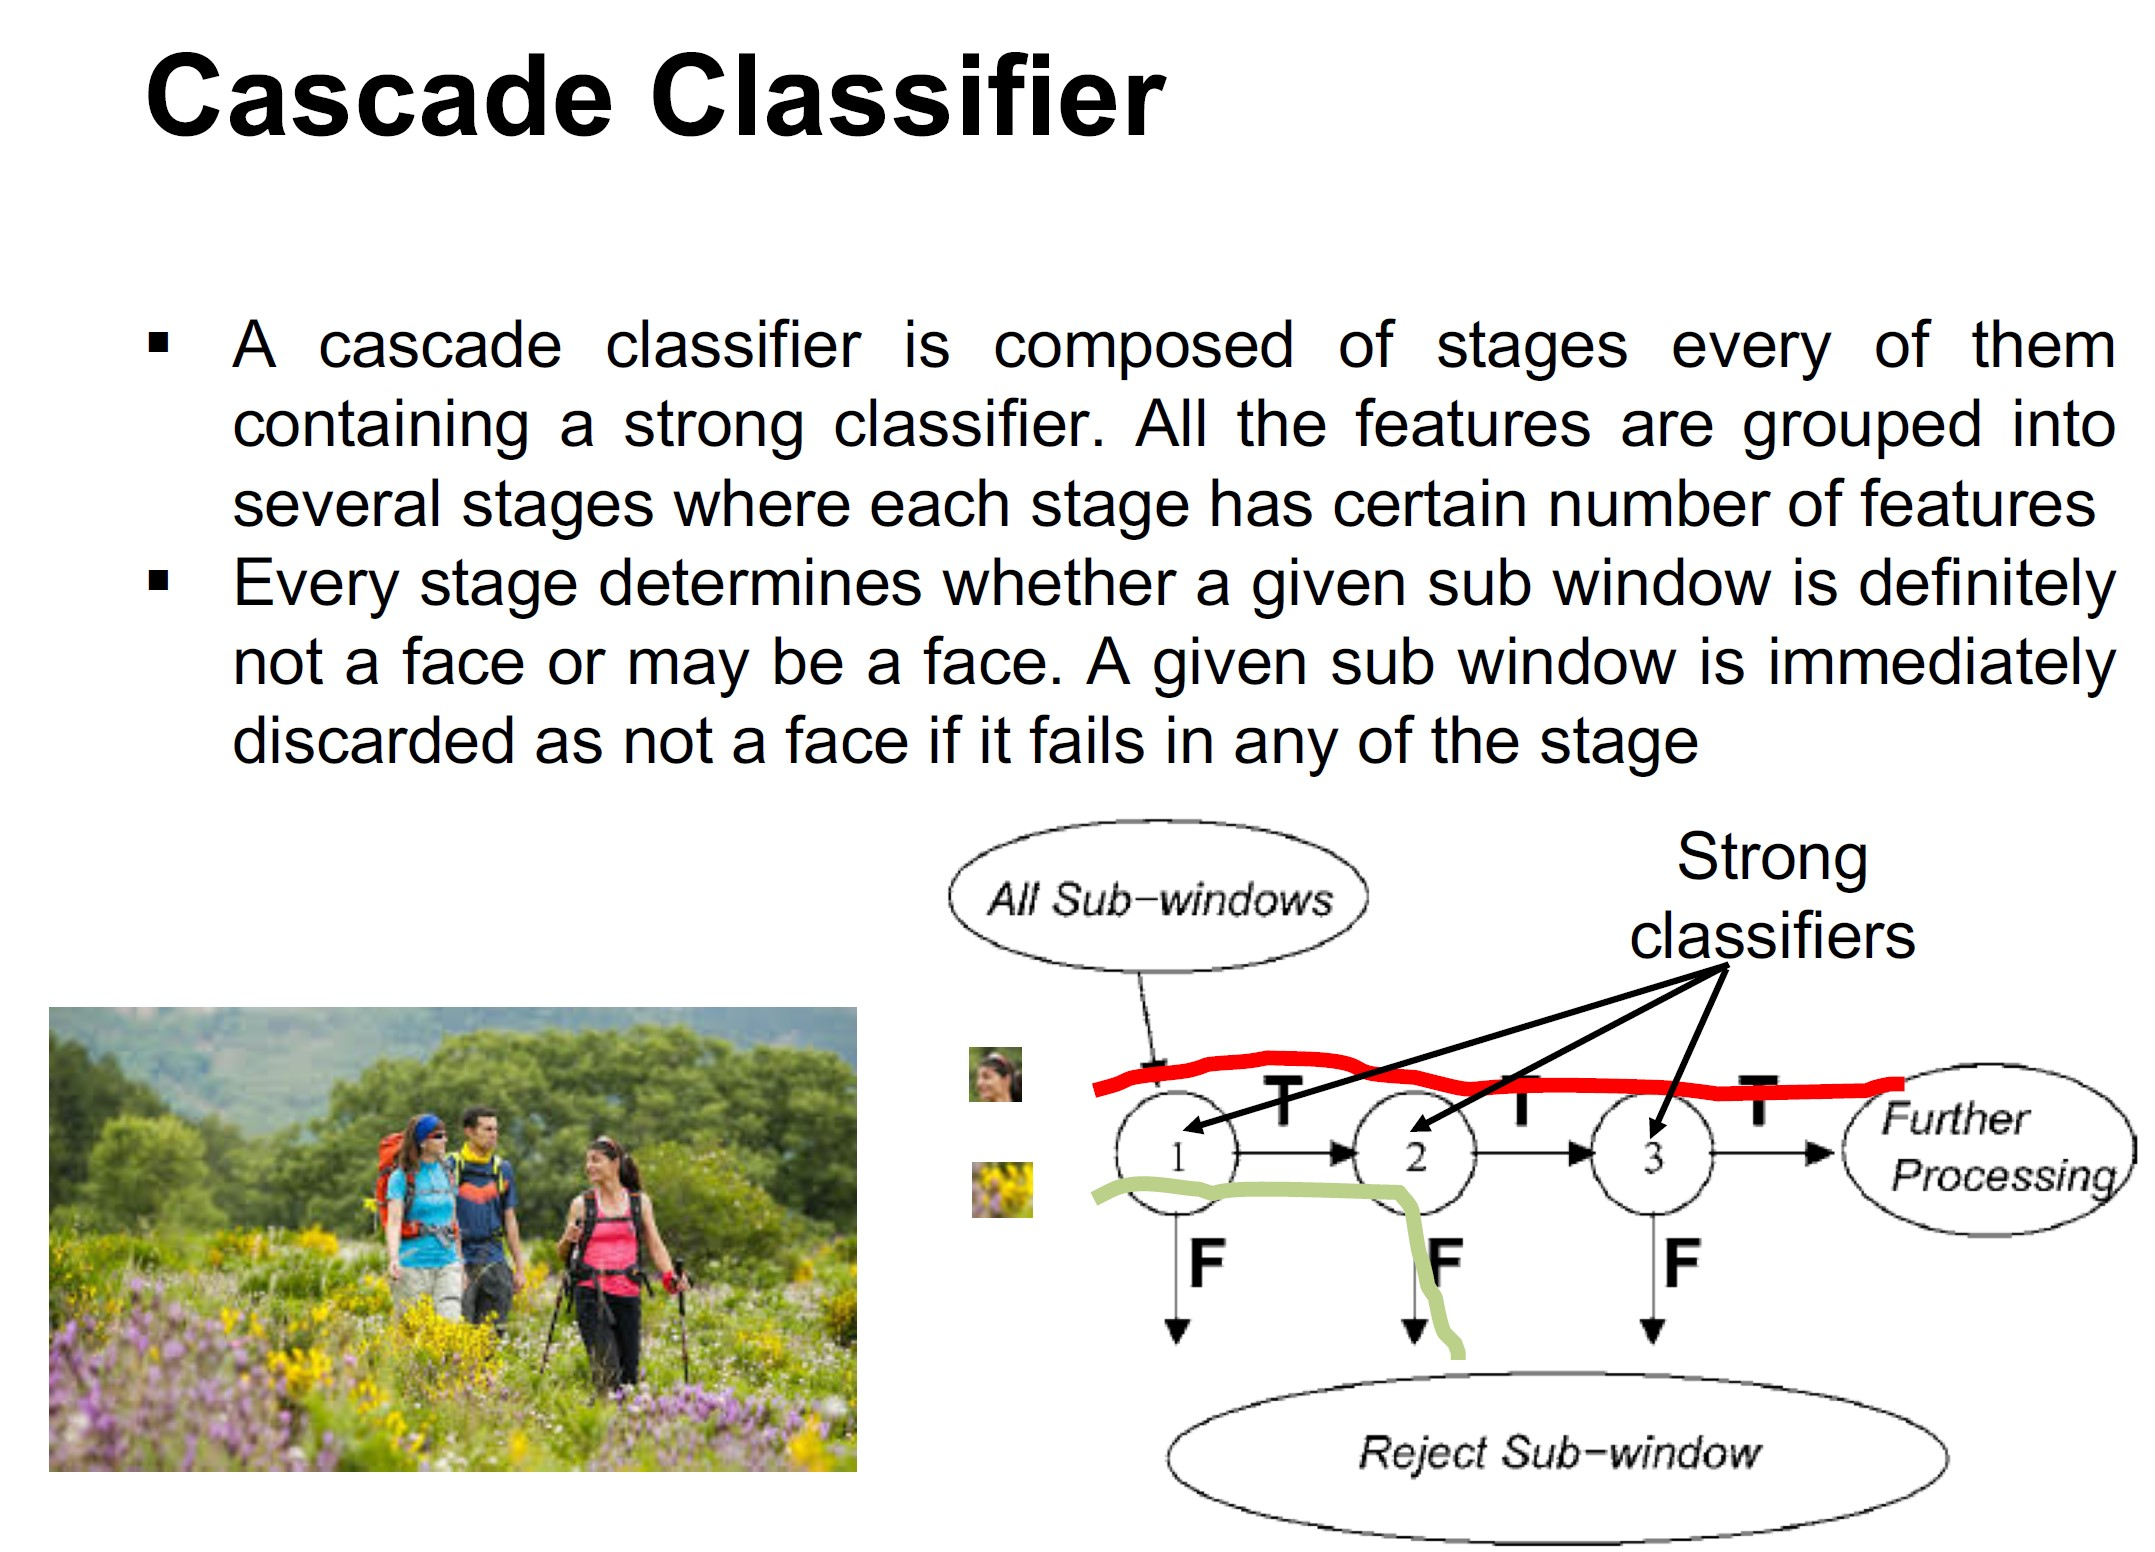
\includegraphics[width=0.75\textwidth]{T1/classifier}
	\caption{Cascade Classifier}
	\label{fig:slideT1}
\end{figure}
\begin{figure}[h]
	\centering
	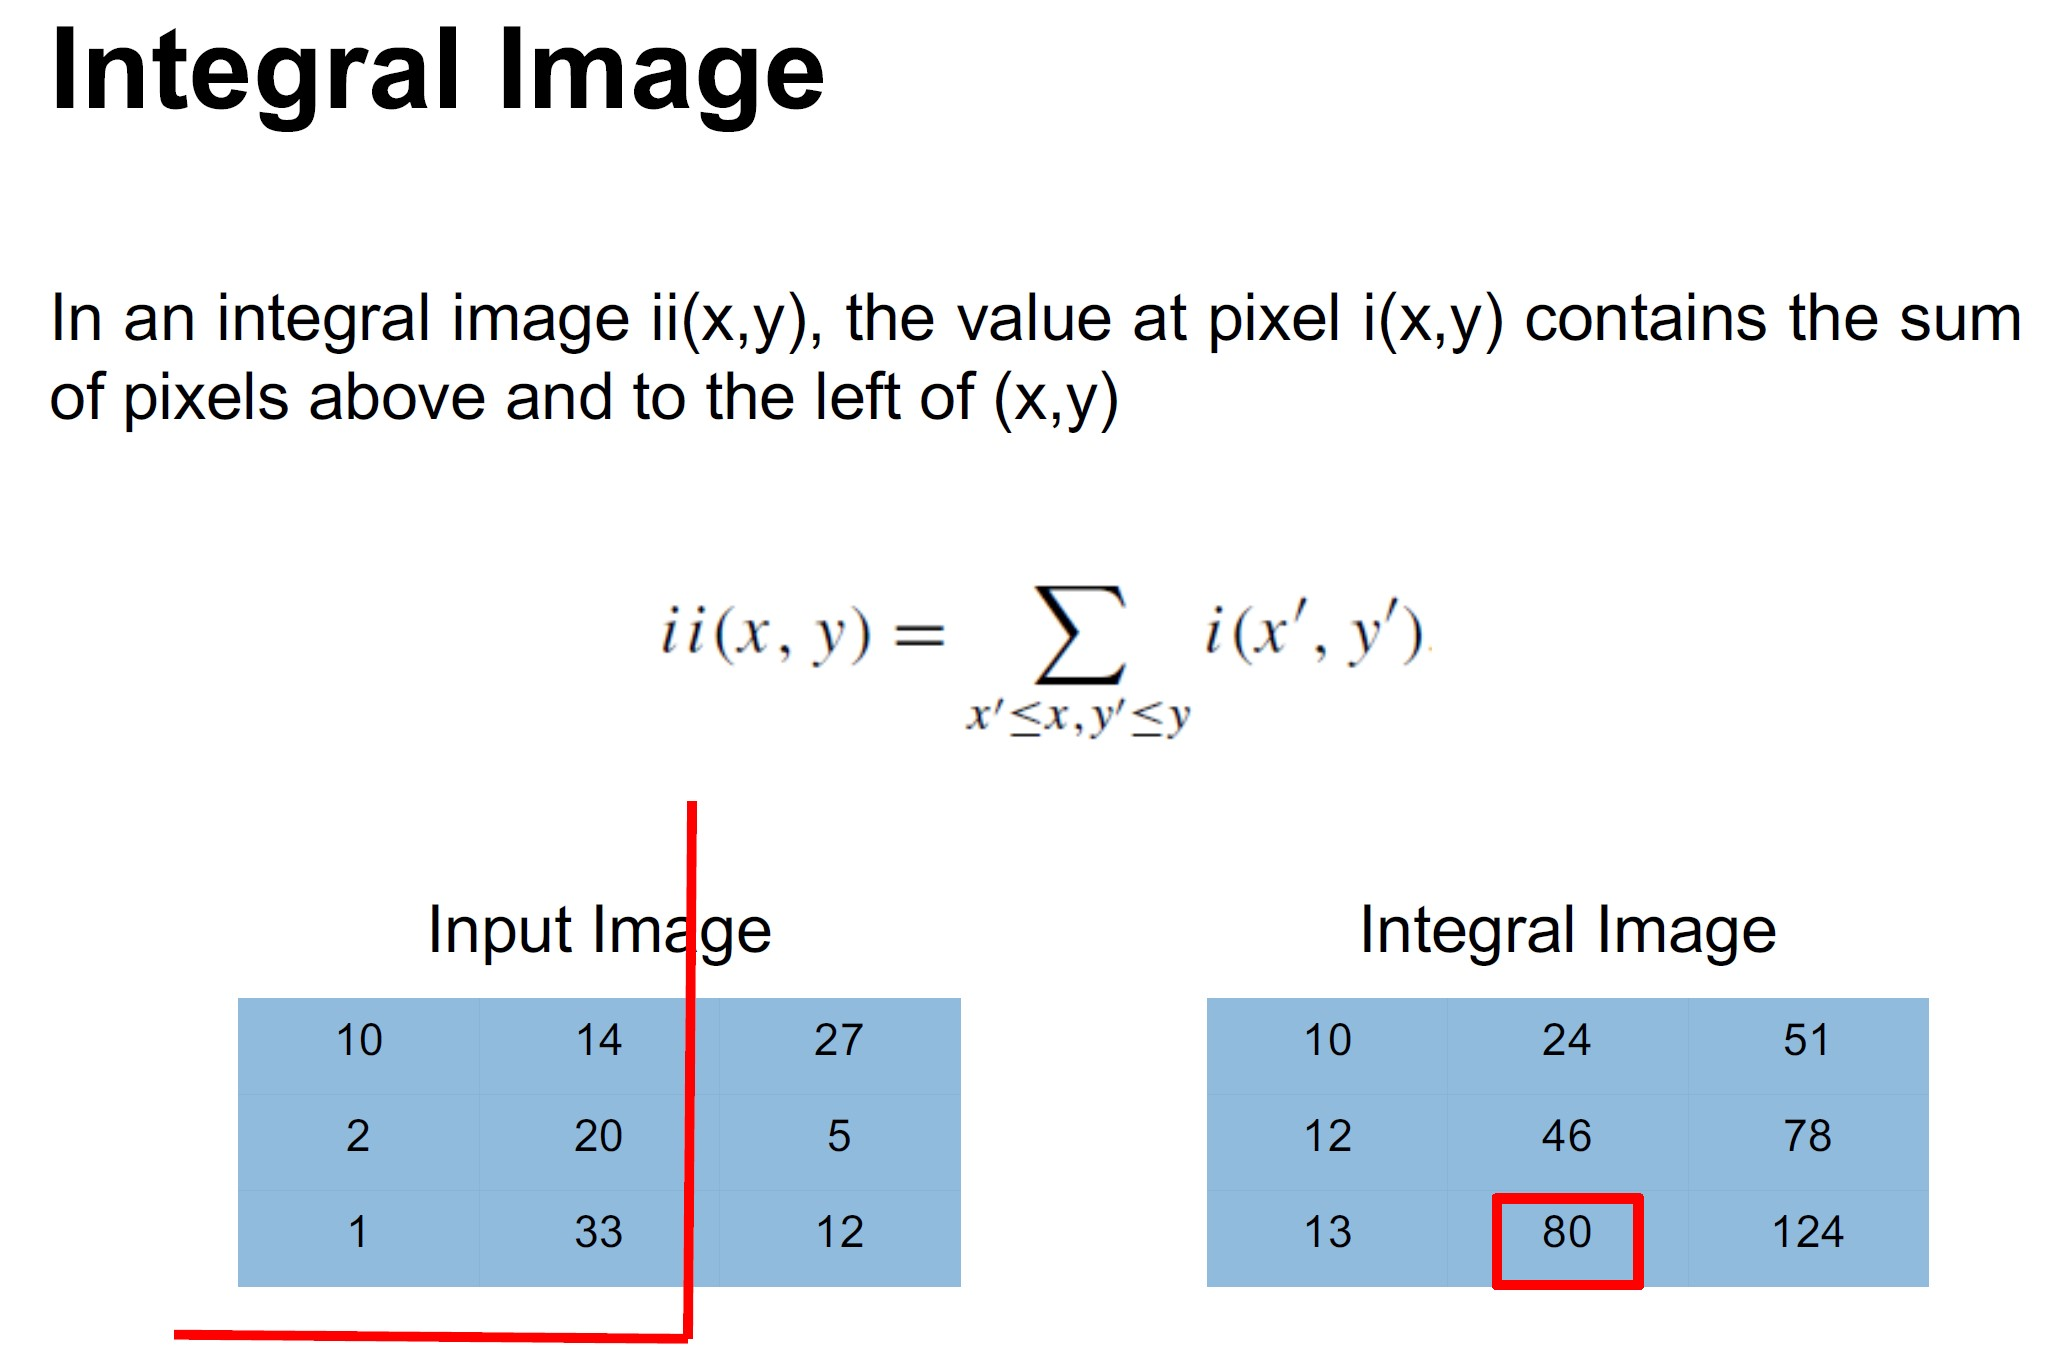
\includegraphics[width=0.75\textwidth]{T1/integral_image}
	\caption{Integral Image calculation}
	\label{fig:integral}
\end{figure}
	\newpage
\subsection{Listing of the Codes}

\begin{lstlisting}[style=Matlab-editor, numbers=left, label={lst:GetIntergralImages},captionpos=b, caption={Code \textbf{GetIntergralImages.m} }]
Picture=im2double(Picture);

if(Options.Resize)
if (size(Picture,2) > size(Picture,1)),
	Ratio = size(Picture,2) / 384;
else
	Ratio = size(Picture,1) / 384;
end
	Picture = imresize(Picture, [size(Picture,1) size(Picture,2) ]/ Ratio);
else
	Ratio=1;
end

if(size(Picture,3)>1),
	Picture=0.2989*Picture(:,:,1) + 0.5870*Picture(:,:,2)+ 0.1140*Picture(:,:,3);
end

s=zeros([size(Picture,1),size(Picture,2)]);
ii=zeros([size(Picture,1),size(Picture,2)]);
for x=1:size(Picture,1)
	for y=1:size(Picture,2)
		if(x==1 && y==1)
			s(x,y)=Picture(x,y);
			ii(x,y)=s(x,y);
		elseif(x==1 && y>1)
			s(x,y)=s(x,y-1)+Picture(x,y);
			ii(x,y)=s(x,y);
		elseif(x>1 && y==1)
			s(x,y)=Picture(x,y);
			ii(x,y)=ii(x-1,y)+s(x,y);
		else
			s(x,y)=s(x,y-1)+Picture(x,y);
			ii(x,y)=ii(x-1,y)+s(x,y);
		end
	end
end
IntegralImages.ii=ii;

IntegralImages.ii=padarray(IntegralImages.ii,[1 1], 0, 'pre');

s2=zeros([size(Picture,1),size(Picture,2)]);
ii2=zeros([size(Picture,1),size(Picture,2)]);
for x=1:size(Picture,1)
	for y=1:size(Picture,2)
		if(x==1 && y==1)
			s2(x,y)=Picture(x,y)^2;
			ii2(x,y)=s(x,y);
		elseif(x==1 && y>1)
			s2(x,y)=s(x,y-1)+Picture(x,y)^2;
			ii2(x,y)=s(x,y);
		elseif(x>1 && y==1)
			s2(x,y)=Picture(x,y)^2;
			ii2(x,y)=ii2(x-1,y)+s2(x,y);
		else
			s2(x,y)=s2(x,y-1)+Picture(x,y)^2;
			ii2(x,y)=ii2(x-1,y)+s2(x,y);
		end
	end
end
IntegralImages.ii2=ii2;

IntegralImages.ii2=padarray(IntegralImages.ii2,[1 1], 0, 'pre');

IntegralImages.width = size(Picture,2);
IntegralImages.height = size(Picture,1);
IntegralImages.Ratio=Ratio;
\end{lstlisting}

\begin{lstlisting}[style=Matlab-editor, numbers=left,label={lst:HaarCasadeObjectDetection},captionpos=b, caption={Code \textbf{HaarCasadeObjectDetection.m} }]
ScaleWidth = IntegralImages.width/HaarCasade.size(1);
ScaleHeight = IntegralImages.height/HaarCasade.size(2);
if(ScaleHeight < ScaleWidth ), 
	StartScale =  ScaleHeight; 
else
	StartScale = ScaleWidth;
end

Objects=zeros(100,4); n=0; 

itt=ceil(log(1/StartScale)/log(Options.ScaleUpdate));

for i=1:itt
	% Current scale
	Scale =StartScale*Options.ScaleUpdate^(i-1);    
	
	if(Options.Verbose)
		disp(['Scale : ' num2str(Scale) ' objects detected : ' num2str(n) ])
	end
	
	w = floor(HaarCasade.size(1)*Scale);
	h = floor(HaarCasade.size(2)*Scale);
	
	step = floor(max( Scale, 2 ));
	
	[x,y]=ndgrid(0:step:(IntegralImages.width-w-1),0:step:(IntegralImages.height-h-1)); x=x(:); y=y(:);
	
	if(isempty(x)), continue; end
	
	[x,y] = OneScaleObjectDetection( x, y, Scale, IntegralImages, w, h, HaarCasade);
	
	for k=1:length(x);
		n=n+1; Objects(n,:)=[x(k) y(k) w h];
	end
end

Objects=Objects(1:n,:);

Objects=Objects*IntegralImages.Ratio;
\end{lstlisting}

\begin{lstlisting}[style=Matlab-editor, numbers=left,label={lst:ObjectDetection},captionpos=b, caption={Code \textbf{ObjectDetection.m} }]
	function Objects = ObjectDetection(Picture,FilenameHaarcasade,Options)
	
	defaultoptions=struct('ScaleUpdate',1/1.2,'Resize',true,'Verbose',true);
	
	functionname='ObjectDetection.m';
	functiondir=which(functionname);
	functiondir=functiondir(1:end-length(functionname));
	addpath([functiondir '/SubFunctions'])

	if(ischar(Picture))
		if(~exist(Picture,'file'))
			error('face_detect:inputs','Image not Found');
		end
	end
	if(~exist(FilenameHaarcasade,'file'))
		error('face_detect:inputs','Haarcasade not Found');
	end

	if(~exist('Options','var')), Options=defaultoptions;
	else
		tags = fieldnames(defaultoptions);
		
	for i=1:length(tags),
		if(~isfield(Options,tags{i})), Options.(tags{i})=defaultoptions.(tags{i}); end
	end
		if(length(tags)~=length(fieldnames(Options))),
			warning('image_registration:unknownoption','unknown options found');
		end
	end

	if(ischar(Picture))
		Picture = imread(Picture);
	end

	HaarCasade=GetHaarCasade(FilenameHaarcasade);

	IntergralImages= GetIntergralImages(Picture,Options);
	
	Objects = HaarCasadeObjectDetection(IntergralImages,HaarCasade,Options);

	if(nargout==0)
		ShowDetectionResult(Picture,Objects);
	end
\end{lstlisting}
	
	





\end{document}     